\documentclass[10pt,twocolumn,letterpaper]{article}
\usepackage{cvpr}
\usepackage{times}
\usepackage{epsfig}
\usepackage{amsmath}
\usepackage{amssymb}
\usepackage{booktabs} % for much better looking tables
\usepackage{array} % for better arrays (eg matrices) in maths
\usepackage{paralist} % very flexible & customisable lists (eg. enumerate/itemize, etc.)
\usepackage{verbatim} % adds environment for commenting out blocks of text & for better verbatim
\usepackage{subfigure} % make it possible to include more than one captioned figure/table in a single float
\usepackage{graphicx}
\usepackage{multirow}
% Include other packages here, before hyperref.
% If you comment hyperref and then uncomment it, you should delete
% egpaper.aux before re-running latex.  (Or just hit 'q' on the first latex
% run, let it finish, and you should be clear).
%\usepackage[pagebackref=true,breaklinks=true,letterpaper=true,colorlinks,bookmarks=false]{hyperref}
\cvprfinalcopy % *** Uncomment this line for the final submission
\def\cvprPaperID{****} % *** Enter the CVPR Paper ID here
\def\httilde{\mbox{\tt\raisebox{-.5ex}{\symbol{126}}}}
% Pages are numbered in submission mode, and unnumbered in camera-ready
\ifcvprfinal\pagestyle{empty}\fi
%use \x, \y, and \w for bold vector forms
\newcommand{\x}{\bold{x}}
\newcommand{\xb}{\bar{x}}
\newcommand{\y}{\bold{y}}
\newcommand{\yb}{\hat{y}}
\newcommand{\w}{\mathbf{w}}
\DeclareMathOperator*{\argmax}{arg\,max}
\begin{document}
%%%%%%%%% TITLE
\title{
Project in CSE 250B\\
Assignment 4: Latent Dirichlet allocation models with Gibbs sampling}
\author{Andreas Landstad, Spencer Bliven, Jonas Hoelzler\\
Computer Science Department\\
University of California, San Diego\\
{\tt\small landstad.andreas@gmail.com, sbliven@ucsd.edu, jonas@hoelzler.de}
}% For a paper whose authors are all at the same institution,
% omit the following lines up until the closing ``}''.
% Additional authors and addresses can be added with ``\and'',
% just like the second author.
% To save space, use either the email address or home page, not both
%\and
%Second Author\\
%Institution2\\
%First line of institution2 address\\
%{\tt\small secondauthor@i2.org}
\maketitle
\thispagestyle{empty}
%%%%%%%%% ABSTRACT
\begin{abstract}
\end{abstract}
%%%%%%%%% BODY TEXT
%INDICES:
% words n=1...N
% features j=1...J
% positions i=1...M_n
% tags k=1...V
%LABELS
% y_n is the correct label
% y' is any label
% \hat{y} is the predicted label
% tags are u or v
% problem: y_1 is ambiguous: i=1 or n=1?
% \xb aka \hat{x} is a vector of letters


\section{Introduction}


\begin{table}
    \begin{tabular}{|l|l|l|}
        \hline
        Topic 1 & Topic 2 & Topic 3 \\
    		\hline    
			  patients   &   system   &   boundary  \\
			  cases   &   problems   &   layer \\
			  ventricular   &   methods   &   wing  \\
			  fatty   &   research   &   mach  \\
			  left   &   scientific   &   supersonic  \\
			  nickel   &   development   &   ratio\\
			  time   &   retrieval   &   wings \\
			  acids   &   general   &   effects\\
			  aortic   &   part   &   velocity\\
			  free   &   language   &   shock\\
			  \hline
    \end{tabular}
\end{table}
%Values
 %   0.0113    0.0083    0.0111
 %   0.0073    0.0069    0.0089
 %   0.0073    0.0067    0.0084
 %   0.0066    0.0065    0.0073
 %   0.0064    0.0063    0.0071
 %   0.0064    0.0059    0.0060
 %   0.0062    0.0058    0.0058
 %   0.0060    0.0055    0.0058
 %   0.0049    0.0049    0.0058
 %   0.0047    0.0048    0.0056


344 Epochs


\begin{figure*}[htbp] 
\centering
   \begin{minipage}{10 cm}
   \centering
    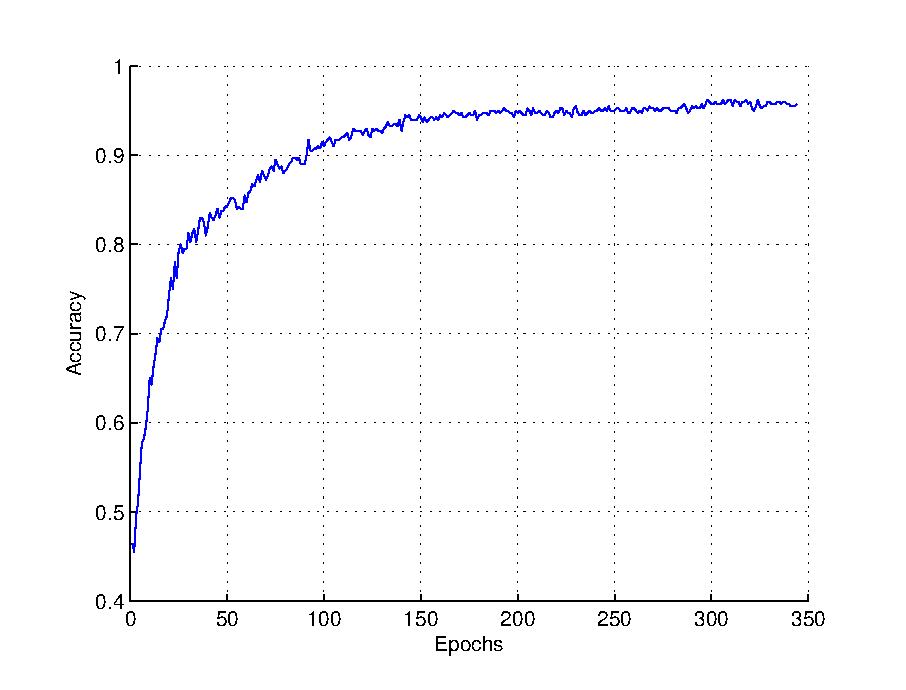
\includegraphics[width=10cm]{images/accuracygrid}
    \end{minipage}
  \caption{Accuracy}
  \label{Labelname}
\end{figure*}


\begin{figure*}[htbp] 
\centering
   \begin{minipage}{10 cm}
   \centering
    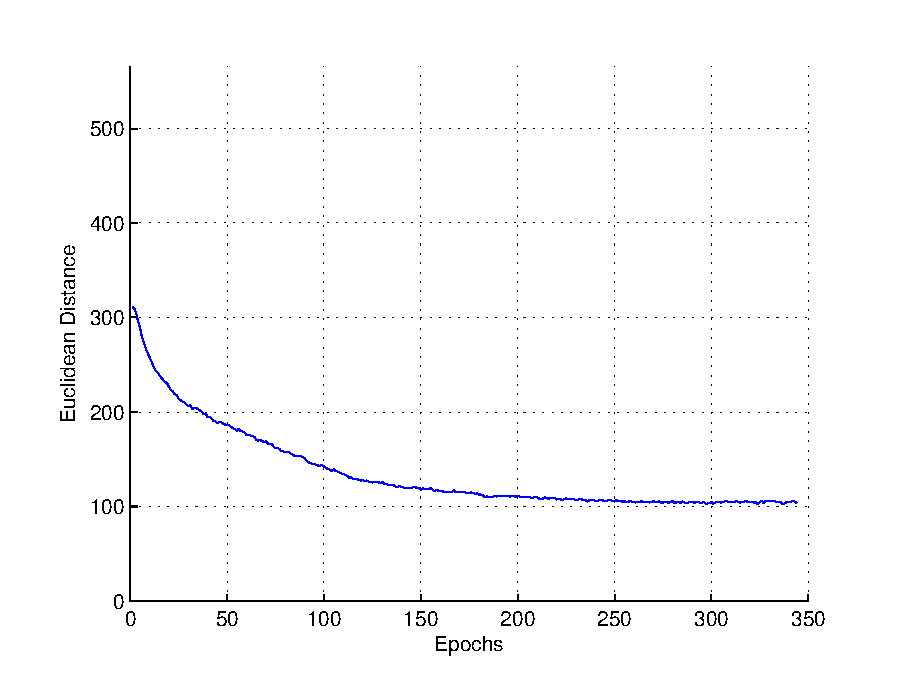
\includegraphics[width=10cm]{images/euclidean}
    \end{minipage}
  \caption{Euclidean Distance to simplex of true labels}
  \label{Labelname}
\end{figure*}


\nocite{blei02,elkan11,bishop06}



{\small
\bibliographystyle{ieee}
\bibliography{egbib}
}
\end{document}
